\section*{Question 2}

The strong form of the boundary value problem given in Assignment 2 is solved using the finite element method with piecewise linear trial and test functions, $\phi(x)$. The problem is analyzed for the mesh sizes
\[
h=\frac{1}{4},\ \frac{1}{8},\ \frac{1}{16},\ \frac{1}{32}.
\]

\subsection*{Finite Element Approximation}

The bar domain $[0,L]$ is discretized into two-node linear finite elements. For each element, the displacement field is approximated using piecewise linear interpolation as
\[
u^h(x)=N_1(x)u_i+N_2(x)u_j,
\]
where $N_1(x)$ and $N_2(x)$ are the linear shape functions and $u_i$, $u_j$ are the nodal displacements of the element.

Using the weak form derived previously, the global finite element system is obtained in the standard form
\[
\mathbf{K}\mathbf{u}=\mathbf{F},
\]
where $\mathbf{K}$ is the global stiffness matrix, $\mathbf{u}$ is the nodal displacement vector, and $\mathbf{F}$ is the global force vector.

For each mesh size, the finite element solution is computed and compared with the exact solution.

\subsection*{Pointwise Comparison with the Exact Solution}

For each mesh size, the following quantities are evaluated:

\begin{itemize}
    \item $u_h(1/3)$
    \item $u_h(1)$
    \item $u_h'(0)$
    \item $u_h'(1)$
\end{itemize}

These values are compared with the corresponding exact solution values. To improve readability and fit, the pointwise results are split into displacement and derivative tables (Tables~\ref{tab:q2_pointwise_disp} and~\ref{tab:q2_pointwise_deriv}).

\begin{table}[H]
\centering
\caption{Pointwise comparison of displacement values.}
\label{tab:q2_pointwise_disp}
\begingroup
\fontsize{13}{15}\selectfont
\renewcommand{\arraystretch}{1.18}
\begin{tabular}{c|cc|cc}
\hline
$h$ & $u_h(1/3)$ & $u(1/3)$ & $u_h(1)$ & $u(1)$ \\
\hline
$1/4$  & $2.680952\times 10^{-2}$ & $2.770581\times 10^{-2}$ & $5.766089\times 10^{-2}$ & $5.817021\times 10^{-2}$ \\
$1/8$  & $2.746309\times 10^{-2}$ & $2.770581\times 10^{-2}$ & $5.803867\times 10^{-2}$ & $5.817021\times 10^{-2}$ \\
$1/16$ & $2.764661\times 10^{-2}$ & $2.770581\times 10^{-2}$ & $5.813703\times 10^{-2}$ & $5.817021\times 10^{-2}$ \\
$1/32$ & $2.769076\times 10^{-2}$ & $2.770581\times 10^{-2}$ & $5.816189\times 10^{-2}$ & $5.817021\times 10^{-2}$ \\
\hline
\end{tabular}
\endgroup
\end{table}

\begin{table}[H]
\centering
\caption{Pointwise comparison of derivative values.}
\label{tab:q2_pointwise_deriv}
\begingroup
\fontsize{13}{15}\selectfont
\renewcommand{\arraystretch}{1.18}
\begin{tabular}{c|cc|cc}
\hline
$h$ & $u_h'(0)$ & $u'(0)$ & $u_h'(1)$ & $u'(1)$ \\
\hline
$1/4$  & $8.700000\times 10^{-2}$ & $1.100000\times 10^{-1}$ & $3.681818\times 10^{-2}$ & $3.333333\times 10^{-2}$ \\
$1/8$  & $9.722222\times 10^{-2}$ & $1.100000\times 10^{-1}$ & $3.500000\times 10^{-2}$ & $3.333333\times 10^{-2}$ \\
$1/16$ & $1.032353\times 10^{-1}$ & $1.100000\times 10^{-1}$ & $3.414894\times 10^{-2}$ & $3.333333\times 10^{-2}$ \\
$1/32$ & $1.065152\times 10^{-1}$ & $1.100000\times 10^{-1}$ & $3.373684\times 10^{-2}$ & $3.333333\times 10^{-2}$ \\
\hline
\end{tabular}
\endgroup
\end{table}

It is observed that the finite element solution approaches the exact solution as the mesh is refined. Both the displacement values and the derivative values become more accurate for smaller values of $h$.

\subsection*{Error Norms}

To quantify the accuracy of the finite element approximation, both the $L^2$ norm and the energy norm of the error are computed for each mesh size.

The $L^2$ norm of the error is defined as
\[
\|e\|_{L^2}=\left(\int_0^L (u-u_h)^2\,dx\right)^{1/2},
\]
where $u$ is the exact solution and $u_h$ is the finite element approximation.

The energy norm of the error is defined as
\[
\|e\|_E=\left(\frac{1}{2}\int_0^L EA(x)\left(u'(x)-u_h'(x)\right)^2\,dx\right)^{1/2}.
\]

The computed error norms are given in Table~\ref{tab:q2_errors}.

\begin{table}[H]
\centering
\caption{Computed $L^2$ and energy norm errors for different mesh sizes.}
\label{tab:q2_errors}
\begingroup
\fontsize{13}{15}\selectfont
\setlength{\tabcolsep}{8pt}
\begin{tabular}{c|cc}
\hline
$h$ & $\|e\|_{L^2}$ & $\|e\|_E$ \\
\hline
$1/4$  & $7.995423\times 10^{-4}$ & $1.708989$ \\
$1/8$  & $2.067882\times 10^{-4}$ & $8.681950\times 10^{-1}$ \\
$1/16$ & $5.218145\times 10^{-5}$ & $4.308346\times 10^{-1}$ \\
$1/32$ & $1.307669\times 10^{-5}$ & $2.119693\times 10^{-1}$ \\
\hline
\end{tabular}
\endgroup
\end{table}
\pagebreak

\subsection*{Convergence Behavior}

To examine the convergence characteristics of the finite element approximation, the values of $\log(\text{error})$ are plotted against $\log(h)$ for both the $L^2$ norm and the energy norm.

\begin{figure}[H]
    \centering
    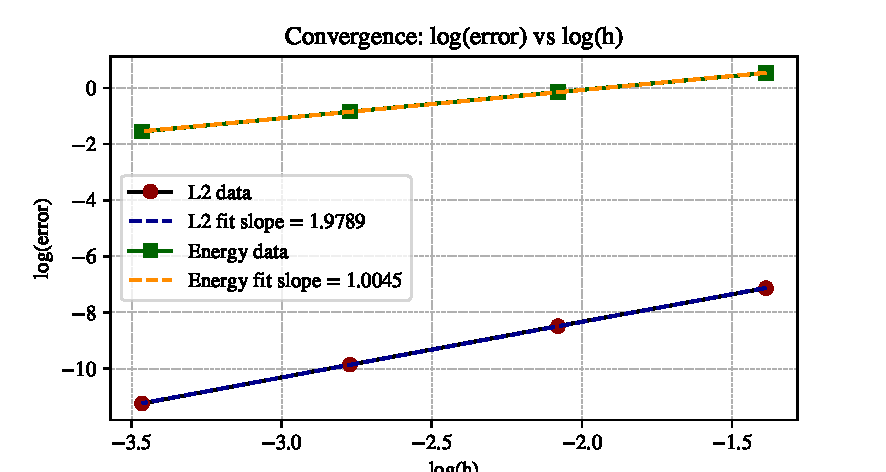
\includegraphics[width=0.9\linewidth]{../ConvergenceError.pdf}
    \caption{Convergence plot of $\log(\text{error})$ versus $\log(h)$ for the $L^2$ and energy norms.}
    \label{fig:q2_convergence}
\end{figure}

The slope of the fitted line in the $\log(\text{error})$--$\log(h)$ plot represents the convergence rate. The obtained slopes are

\[
\text{Slope in }L^2\text{ norm} = \boxed{1.978886},
\qquad
\text{Slope in energy norm} = \boxed{1.004453}.
\]

The results show that the $L^2$ norm converges approximately at second order, while the energy norm converges approximately at first order. This behavior is consistent with the theoretical convergence properties of linear finite elements.
\pagebreak

\subsection*{Finite Element Displacement Response}

The finite element displacement solutions for all mesh sizes are plotted together with the exact solution in Figure~\ref{fig:q2_displacement}.

\begin{figure}[H]
    \centering
    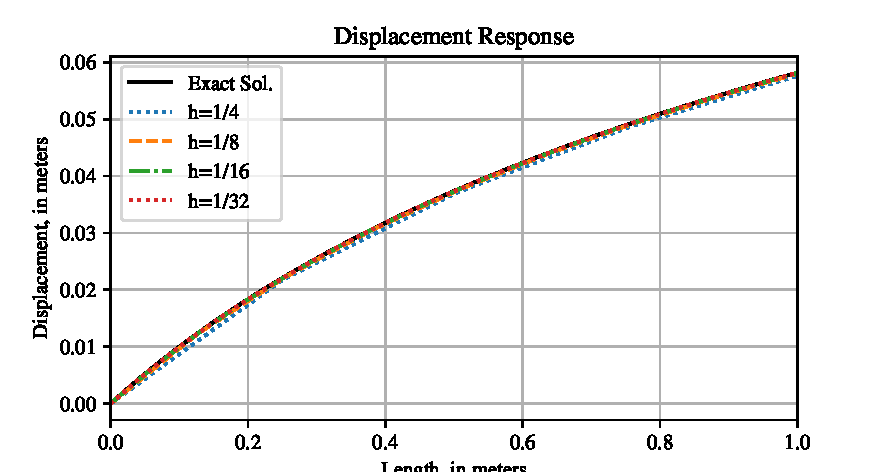
\includegraphics[width=0.9\linewidth]{../uResponse.pdf}
    \caption{Finite element displacement solutions for different mesh sizes together with the exact solution.}
    \label{fig:q2_displacement}
\end{figure}

It can be seen that the finite element displacement solution becomes progressively closer to the exact solution as the mesh is refined.
\pagebreak

\subsection*{Derivative of the Displacement Response}

The first derivative of the finite element solution is plotted together with the derivative of the exact solution in Figure~\ref{fig:q2_derivative}.

\begin{figure}[H]
    \centering
    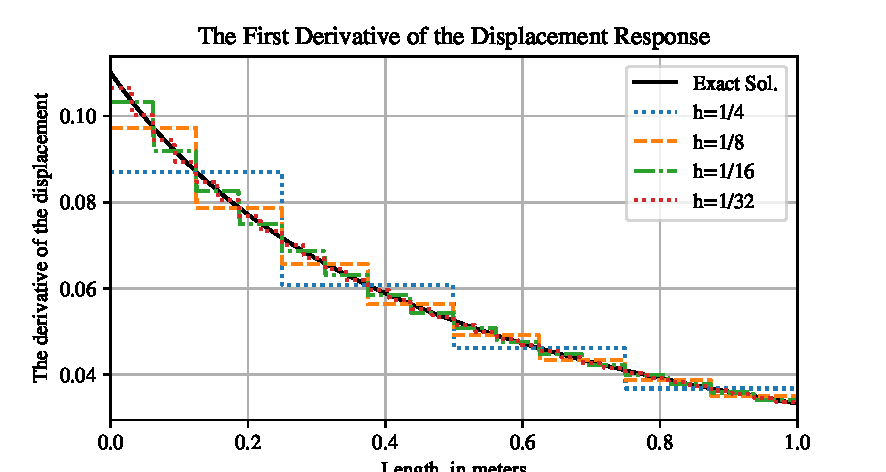
\includegraphics[width=0.9\linewidth]{../uPrimeResponse.pdf}
    \caption{First derivative of the finite element solution for different mesh sizes together with the derivative of the exact solution.}
    \label{fig:q2_derivative}
\end{figure}

Since linear finite elements are used, the derivative of the finite element solution is piecewise constant over each element. Therefore, the approximation of the derivative is less smooth than the displacement field. Nevertheless, the derivative approximation improves as the mesh is refined.

\subsection*{Discussion of Results}

The results demonstrate clear convergence of the finite element solution toward the exact solution as the mesh is refined. The $L^2$ error decreases by approximately a factor of four when the mesh size is halved, indicating second-order convergence, while the energy norm decreases by approximately a factor of two, confirming first-order convergence, both consistent with theoretical expectations for linear finite elements. The displacement field is captured accurately even on coarse meshes, whereas the derivative exhibits slower convergence due to its piecewise constant representation within each element. This behavior arises directly from the use of linear shape functions, which enforce constant strain over each element. Overall, the numerical results validate both the formulation and implementation of the finite element method for this problem.

\subsection*{Code Repository}

GitHub link: \url{https://github.com/ImranMETU/CE526_Assignment3}